\graphicspath{{chapters/6.Chapter_4/figures/}}

\begin{savequote}[75mm]
In biology, nothing is clear, everything is too complicated, everything is a mess, 
and just when you think you understand something, you peel off a layer and find 
deeper complications beneath. Nature is anything but simple.
	\qauthor{- Richard Preston: The Hot Zone}
\end{savequote}

\chapter{RNAi Analyses}


\section{Introduction}

RNAi is a highly useful experimental methodology through which
many biological hypotheses can be tested.





23nt siRNA from Dcr1 in \textit{P. tetaurelia} \citep{Lepere2009}



\subsection{RNAi pathway in \textit{Paramecium} sp.}

Is there significant cross-talk between endosymbiont and host? - is this why RNAi doesn't seem to work

What of the required RNAi components from Marker are present in genome and transcriptome host bins

What is the phylogeny of these components compared to other Paramecium/ciliate species?

eDicer experiment results - what is the overlap with host orthologs of known yeast lethal genes

rnai as cross-kingdom communication \citep{Weiberg2015}

FIGURE 5. Dating of genome duplication events





%\begin{figure}
%    \includegraphics[]{}
%    \caption{Redrawing of known \textit{Paramecium} RNAi components/pathway from the marker paper}
%    \label{fig:rnai_components}
%\end{figure}


\section{Aims}

Induce RNAi based knock-down using transformed bacterial vectors.

RNAi via microinjection

Identify required components for endogenous or exogenous RNAi in \textit{P. bursaria} CCAP 1660/12 from transcriptome and genome

Investigate the possiblity of "host" - "endosymbiont" collision as a reason for disabling.


\section{Methods}

\subsection{RNAi feeding experiments}

Methods modified from ParameciumDB 


PGM was identified in the genomic contigs (see chapter 1).

\begin{table}
    \begin{tabular}{|c|c|c|c|c|}
        \hline
    \textbf{Gene} & \textbf{Function} & \textbf{RNAi phenotype in}      & Vector Design & Reference \\
                  &                   & \textbf{\textit{P. tetaurelia}} &               &           \\
        \hline
        \textit{epi2} & Epiplasmin & ``Monstrous'' cells  & 500bp via \textit{Pst}I and \textit{Hind}III & \citep{Damaj2009} \\
        NSF & Membrane fusion factor & Lethal & 500bp via \textit{Pst}I and \textit{Hind}III & \citep{Galvani2002} \\
        pTMB.422c & Binding protein & Lethal & 500bp via \textit{Pst}I and \textit{Hind}III & \citep{Nowack2011} \\
        \textit{bug22} & Basal body/ciliary protein & Slow swimming and death & 313bp via \textit{Xba}I and \textit{Hind}III & \citep{Laligne2010} \\
        BBS7 & Ciliary ion transport & Fewer, shorter ciliar & 486bp via \textit{Xho}I and \textit{Hind}III & \citep{Valentine2012} \\
        PGM & PGM endonuclease & Post-autogamous cells unable to resume normal growth & 500bp via \textit{Pst}I and \textit{Hind}III & \citep{Baudry2009} \\
        \hline
    \end{tabular}
    \caption{Details of RNAi vectors used.  All constructs were cloned into a L4440 vector and used an Ampicillin resistance market}
    \label{tab:rnai_vecs}
\end{table}


\subsection{RNAi microinjection}

\subsection{Analysis of RNAi pathway}

\subsubsection{Genomic survey for components}

BLASTP using sequences from Marker against transcriptome
and genome

\begin{table}
    \centering
    \begin{tabular}{|c|c|c|c|}
        \hline
        \textbf{Gene} & \textbf{\textit{P. tetaurelia} Accession} & \textbf{Length} & \textbf{Role} \\
        \hline
        Rdr1 & PTETG8500012001 & 4319 & Exo\\
        Rdr2 & GSPATG00036857001 & 4162 & Exo and Endo\\
        Rdr3 & GSPATG00006401001 & 3292 & Endo \\
        Cid1 & PTETG9100013001 & 1051 & Exo\\
        Cid2 & PTETG13400003001 & 1083 & Exo and Endo \\
        PSD1 & PTETG600032001 & 2084 & Exo \\
        Dcr1 & GSPATG00021751001 & 5394 & Exo and Endo\\
        Ptiwi12 & GSPATG00001709001 & 2315 & Exo \\
        Ptiwi13 & PTETG4800007001 & 2483 & Exo and Endo \\
        Ptiwi14 & PTETG16300003001 & 2428 & Endo \\
        Ptiwi15 & GSPATG00005370001 & 2315 & Exo \\
        \hline
    \end{tabular}
    \caption[RNAi pathway components from Marker]{\citep{Marker2014}}
\end{table}



\subsubsection{Phylogenetic analysis of RNAi pathway}




\section{Results}

\subsection{RNAi feeding experiments}

Fail

\subsection{RNAi microinjection experiment}

Fail

\subsection{RNAi required components}

BLASTX

%Cid1 NODE525 - 17.6kb e-30/-50 40/50% id    356-943, 86-123
%Cid2 NODE525 - 17.6kb e-45 35-54% id    281-1009, 51-284
%Cid3 NODE525 - 17.6kb e-25 30-45% id    150-1179, 150-303
%PSD1 no real hits
%DCR1 Node3133, Node1758, e-140, e-100
%Rdr1 Node2867, NODE374, 0, e-77, 3046-326, (Rdr1 in ptet node2867 top hit reciprocal)
%Rdr2 Node2867, -134 3046, 967
%Rdr3 No hit


\subsubsection{Cid}

%\begin{figure}
%    \includegraphics[width=\textwidth]{cid1_2_3.pdf}
%    \caption[Bayesian and ML Phylogeny of Cid Cid1 and Cid2]{Bayesian
%    and Likelihood phylogeny of CID components}
%    \label{fig:cid_phlyo}
%\end{figure}





\section{Discussion}

\subsection{Exogenous RNAi is non-functional in \textit{P. bursaria} CCAP 1660/12}

PSD1 is totally absent. 

Degenerate PCR was attempted using sequences from \textit{P. tetaurelia} and 
the other \textit{aurelia}




\subsection{Endogenous RNAi is methodologically difficult}


While RNAi by microinjection repeatedly failed there is a still a high possibility
that this is more related to the methodological difficulty of this technique rather than
necessarily any 
\cref{fig:microinjection_nucleus}

\begin{figure}
    \includegraphics[width=\textwidth]{microinjection_hard.pdf}
    \caption{}
    \label{fig:microinjection_nucleus}
\end{figure}


\subsection{Deactivation requires confirmation}




\subsection{Endosymbiont ``collision'' hypothesis}

Hypothetically, one explanation for the deactivation/loss
of RNAi in \textit{P. bursaria} CCAP 1660/12.

- need to confirm 




\section{Conclusions}

RNAi induced phenotypes could not be created in \textit{P. bursaria} CCAP1660/12
by either feeding experiments or direct transgene microinjection. 

Therefore, assembled transcriptomic and genomic data from \textit{P. bursaria}
CCAP 1660/12 and YADG1N were analysed for factors identified as essential in the function
of these pathways in \textit{P. tetaurelia} \citep{Marker2014}. 

\begin{figure}
    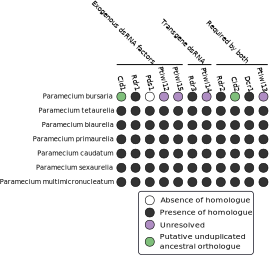
\includegraphics[width=\textwidth]{RNAi_factors_summary_figure.pdf}
    \caption[Summary of RNAi Factors Presence]{Summary of the discovery
    of RNAi figures in \textit{P. bursaria}}
    \label{fig:rnai_summary}
\end{figure}

Two proteins essential for the function of the exogenous dsRNA induced
RNAi pathway in \textit{P. tetaurelia}, Psd1 and Rdr1, were not found in the partial genome and transcriptome 
of \textit{P. bursaria} CCAP 1660/12 or the transcriptome of \textit{P. bursaria} YADG1N.
This suggests that this pathway may not be active/present in \textit{P. bursaria}.
Either, 


However, assuming the likely pre-duplication orthologue of Cid2 and the necessary 
unresolved Ptiwi's are functional
in the transgene dsRNA pathway of \textit{P. bursaria}
then this pathway is theoretically active.  Unfortunately, methodological
difficulties in microinjection have thus far failed to generate RNAi-induced
phenotypes.
